\chapter{Fonctionnement du programme}
    \section{Interface graphique}
        \begin{figure}[h]
            \begin{center}
                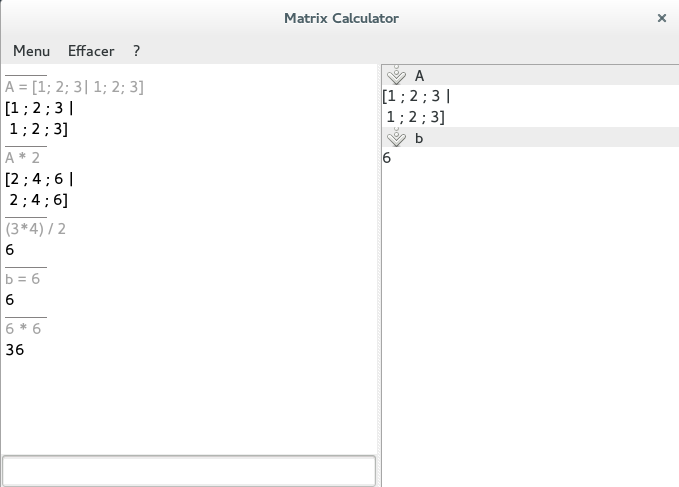
\includegraphics[scale=0.5]{interface.png}
            \end{center}

            \caption{Interface du programme}
            \label{Interface du programme}
        \end{figure}

    L'interface est composée d'un champ d'entrée de sélection, d'une zone d'affichage comprenant les expressions entrées et leurs résultat (ou erreur) ainsi qu'une gestionnaire de variable.
    \\ Dans la partie principale, l'expression entrée par l'utilisateur est en gris et les erreurs, s'il y en a, sont affichées en rouges. et le resultat retournée par son expression en noir. Chaque expression est séparée par une ligne noire.
    \\ Il est possible à l'aide des flèches de remonter ou redescendre dans l'historique des entrées, en ayant pris soin de sélectionner la zone de texte d'entrée.
 

    \newpage

    \section{Fonctionnalités}
        \paragraph{}
            Les variables et leur contenu sont affichés en temps réel sur la droite. L'utilisateur peut vider le contenu des variables en cliquant droit sur l'une d'elle, un menu contextuel apparaît et offre la possibilité de la supprimer.
            \\ En cliquant simplement sur le nom de la variable, il est possible d'afficher ou de cacher sont contenu.
            \\ La suppression des variables, ainsi que celle de l'historique est disponible dans le menu ``effacer''.

        \paragraph{}
            L'état actuel du programme (contenu des variables ainsi qu'historique des entrées) peut être sauvegardé dans un fichier à l'aide du raccourcis clavier Ctrl+S ou dans le menu ``Menu''.
            \\ De la même manière, un état précédent du programme peut être récuperé en ouvrant un fichier avec le raccourcis Ctrl+O ou dans le menu ``Menu''.

        \paragraph{}
            L'assignation à une variable se fait de la manière suivante: \[nomVariable = [valeur]\] 
            \\ La valeur peut être un scalaire, la résultante d'une fonction ou une matrice.
            \\ Les fonctions implémentées sont :
            \begin{enumerate}
                \item Le déterminant d'une matrice \[det([matrice])\]
                \item L'inverse d'une matrice \[inv([matrice])\]
                \item La résolution d'équation linéaires (scalaires ou matricielles): \[solve([A], [B])\] 
            \end{enumerate}
            La syntaxe de définition d'une matrice est la suivante (pour une matrice 2x2)
                \[ [ [valeur]; [valeur] | [valeur]; [valeur] ]\]
            Le ``;'' est le séparateur de colonne et ``|'' le séparateur de ligne.
